 \documentclass[book.tex]{subfiles}
\begin{document}


\section{Audio and Heartbeat} 
\label{audio_and_heartbeat}
The audio and heartbeat system runs concurrently with the rest of the program. On an operating system supporting neither multi-processes nor threads this means using interrupts to stop normal execution and perform tasks on the side.\\
\par
The idea is to configure the hardware to trigger a hardware interrupt at a regular interval. This interrupt is caught by a system called PIC which transforms it into a software interrupt, or IRQ. The software interrupt ID is used as an offset in a vector to look up a function belonging to the engine. At this point, the CPU is stopped (a.k.a: interrupted) from doing whatever it was doing (likely running the 2D renderer), and it starts running the interrupt handler which is called an ISR\footnote{Interrupt Service Routine}. We now have two systems running in parallel.\\
\par
\begin{figure}[H]
  \centering
  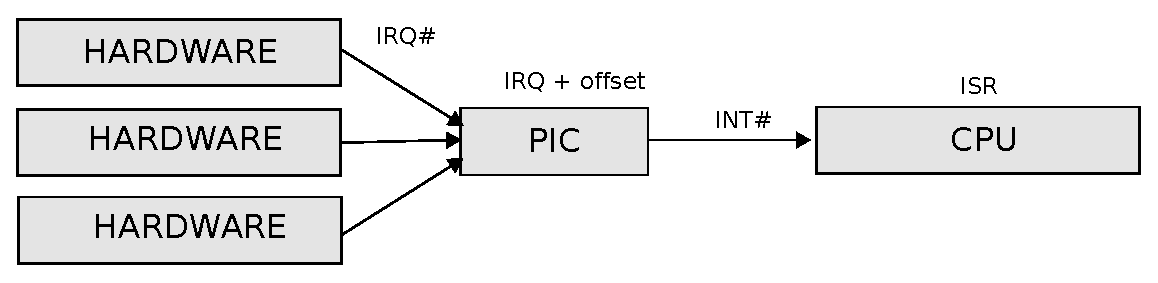
\includegraphics[width=\textwidth]{imgs/drawings/irqs/explanationsvg.eps}
  \caption{Hardware interrupts are translated to software interrupt via the PIC.}
\end{figure}
\par
 Since interrupts keep triggering constantly from various sources, an ISR must choose what should happen if an IRQ is raised while it is still running. There are two options.  The ISR can decide it needs a "long" time to run and disable other IRQs via the IMR \footnote{Interrupt Mask Register}. This path introduces the problem of discarding important information such as keyboard or mouse inputs.\\
 \par
 Alternately, the ISR can decide not to mask other IRQs and do what it is supposed to do as fast as possible so as to not delay the firing of other important interrupts that may lose data if they aren't serviced quickly enough. Keen Dreams uses the latter approach and keeps tasks in its ISR very small and short. 

\subsection{IRQs and ISRs}
The IRQ and ISR system relies on two chips: the Intel 8254 which is a PIT\footnote{Programmable Interval Timer} and the Intel 8259 which is a PIC\footnote{Programmable Interrupt Controller}. The PIT features a crystal oscillating in square waves. The PIT contains three channels, each connected with a counter. On each period, it decrements its three counters. Counter \#2 is connected to the buzzer and generates sounds. Counter \#1 is connected to the RAM in order to automatically perform something called "memory refresh"\footnote{Without frequent refresh, DRAM will lose its content. This is one of the reasons it is slower and SRAM is preferred in the caching system.}. Counter \#0 is connected to the PIC. 
When counter \#0 hits zero it generates an IRQ\footnote{Interrupt Request Line: Hardware lines over which devices can send interrupt signals to the CPU.} and sends it to the PIC.\\

\
\par
\begin{figure}[H]
  \centering
  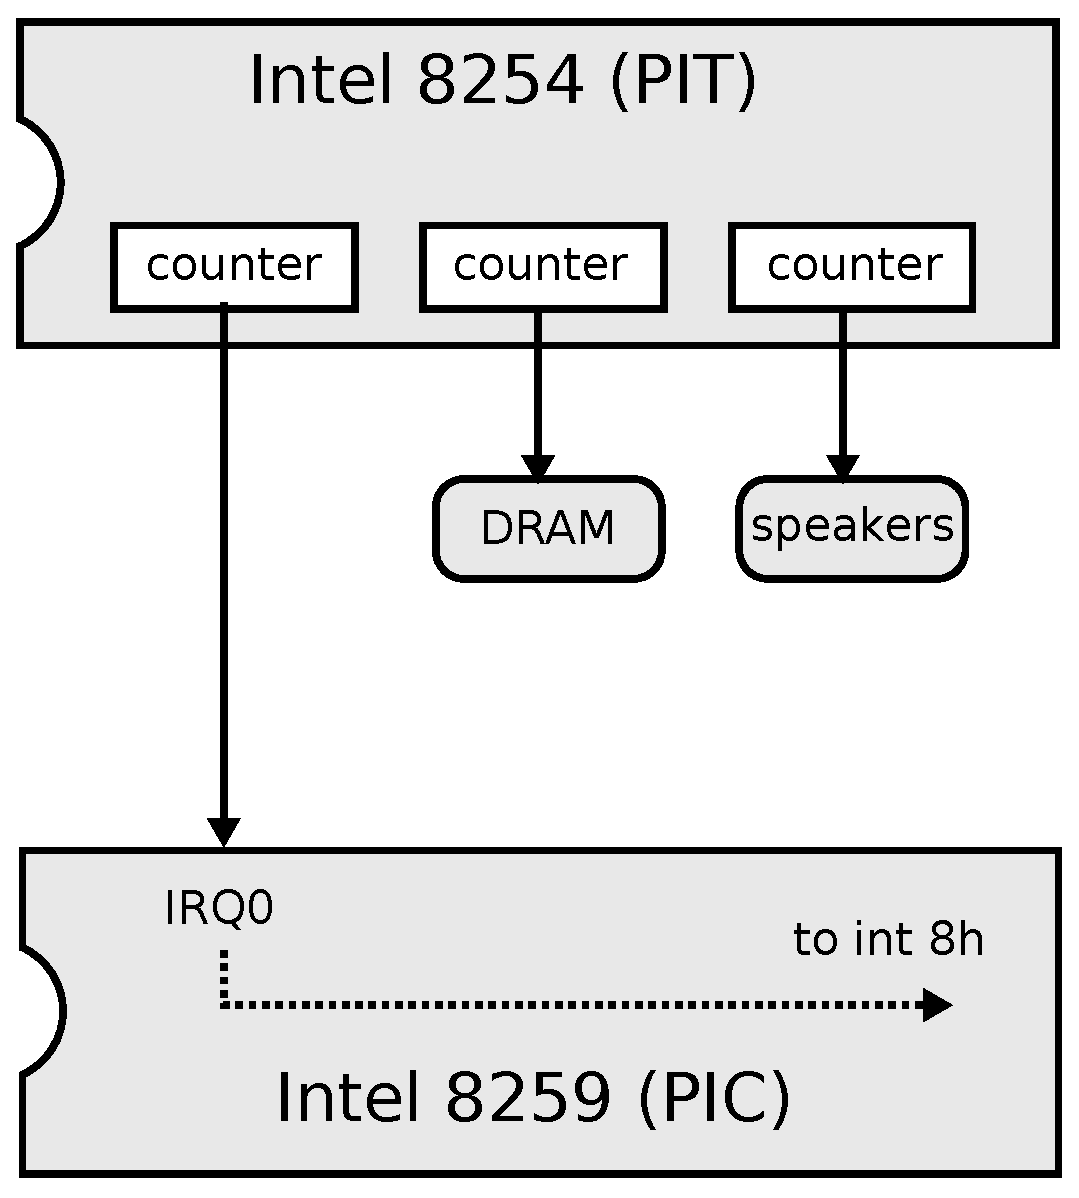
\includegraphics[width=.65\textwidth]{imgs/drawings/heatbeats.eps}
  \caption{Interactions between PIT and PIC.}
\end{figure}
\par

The PIC's hardware IRQ-0 to IRQ-8 are mapped to the Interrupt Vector starting at Offset 8 (resulting in mapping to software interrupts INT08 to INT0F). \pagebreak

\begin{figure}[H]
	\centering
	\begin{tabularx}{\textwidth}{ l p{.5\textwidth}  }
	  \toprule
	  \textbf{I.V.T Entry \#} & \textbf{Type} \\ \bottomrule

	  00h	&	CPU divide by zero \\
01h	&	Debug single step \\
02h	&	Non Maskable Interrupt \\
03h	&	Debug breakpoints \\
04h	&	Arithmetic overflow \\
05h	&	BIOS provided Print Screen routine \\
06h	&	Invalid opcode \\
07h	&	No math chip \\
08h & IRQ0, System timer \\
09h & IRQ1, Keyboard controller \\
0Ah & IRQ2, Bus cascade services for second 8259 \\
0Bh & IRQ3, Serial port COM2 \\ 
0Ch & IRQ4, Serial port COM1 \\
0Dh & IRQ5, LPT2, Parallel port (HDD on XT) \\
0Eh & IRQ6, Floppy Disk Controller \\
0Fh & IRQ7, LPT1, Parallel port \\
10h & Video services (VGA)\\
11h & Equipment check \\
12h & Memory size determination \\
		\bottomrule
	\end{tabularx}
	\caption{The Interrupt Vector Table (entries 0 to 18).}
\end{figure}
Notice \#8 which is associated with the System timer and usually updates the operating system clock at 18.2 ticks per second. Because IVT \#8 was hijacked, the operating system clock is not updated while Commander Keen runs. Upon exiting the game, DOS will run late by the amount of time played.\\
\par
Using these two chips and placing its own function at Interrupt Vector Table (IVT) \#8, the engine can stop its runtime at a regular interval, effectively implementing a subsystem running concurrently with everything else.\\
\par
IVT \#8 is also responsible for turning off the floppy disk motor after a disk read or write operation. The timer interrupt maintains a disk motor shutoff counter which is decreased every time the timer interupt is called. When the counter reaches 0, the interrupt timer shuts off the disk motor. But since IVT \#8 is hijacked, this function is never called and the floppy disk motor keeps running forever. Although this is not an issue, it might give the user the idea that the floppy is still transferring data.\\
\par

So solve the problem, the timer interrupt subsytem performs a check if any of the disk motors is still running. Checking the status of the disk motors can be done via the BIOS Data area, which is a section of memory located at segment \cw{0040h} and stores many variables indicating information about the state of the computer\footnote{For a full overview of BIOS Data Area see https://www.stanislavs.org/helppc/bios\_data\_area.html.}:
\begin{itemize}
  \item BIOS data address \cw{40h:3Fh} contains the motor status, where bit 0 flags if the disk 1 motor is on and bit 1 if disk 2 motor is on.
  \item BIOS data address \cw{40h:40h} holds the disk motor shutoff counter, used by the original timer interrupt.
\end{itemize}

The interrupt subsystem validates if any of the two disk motors is runnning and then checks and decrements the disk motor shutoff counter. In case the shutoff counter is 0 or 1 the original timer interrupt is being called, until both disk motors are turned off.
\\

\par
\begin{minipage}{\textwidth}
\lstinputlisting[language=C,morekeywords={longword}]{code/disk_motor.c}
\end{minipage}\\
\par


\subsection{PIT and PIC}
The PIT chip runs at 1.193182 MHz. This initially seems like an odd choice from the hardware designers, but has a logical origin. In 1980 when the first IBM PC 5150 was designed, the common oscillator used in television circuitry was running at 14.31818 MHz. As it was mass produced, the TV oscillator was very cheap so utilizing it in the PC drove down cost. Engineers built the PC timer around it, dividing the frequency by 3 for the CPU (which is why the Intel ran at 4.7MHz), and dividing by 4 to 3.57MHz for the CGA video card. By logically ANDing these signals together, a frequency equivalent to the base frequency divided by 12 was created. This frequency is 1.1931816666 MHz. By 1990, oscillators were much cheaper and could have used any frequency but backward compatibility prevented this.\\

\subsection{Interrupt Frequency}
Each counter on the PIT chip is 16-bit, which is decremented after each period. An IRQ is generated and send to the PIC whenever the counter wraps around after 2\textsuperscript{16} = 65,536 decrements. So at default, the interrupts are generated at a frequency of 1.19318MHz / 65,536 = 18.2Hz. Some programs require a faster period than the 18.2 interrupts/second standard rate (for example, execution profilers). So they reprogram the timer by changing the counter value.\\
\par
\begin{minipage}{\textwidth}
\lstinputlisting[language=C,morekeywords={longword}]{code/set_timer.c}
\end{minipage}\\
\par

\textbf{\underline{Trivia :}} Note that \cw{SDL\_SetTimer0} is using a frequency of 1.192755MHz, instead of the PIT documented 1.193182MHz. Most likely the value is based on 18.2 interrupts per second * 65,536 = 1192755Hz.\\

\par
So the engine can decide at what frequency to be interrupted, depending on the type of sound/music it needs to play and what devices will be used. As a result, two frequencies are defined: 
\begin{enumerate}
\item Running at 140Hz to play sound effects and music on the PC beeper, AdLib and SoundBlaster.
\item Running at 700Hz to play sound effects and music on Disney Sound Source.
\end{enumerate}
\par
\begin{minipage}{\textwidth}
\lstinputlisting[language=C]{code/set_sound_mode.c}
\end{minipage}
\par












\subsection{Heartbeats}
Each time the interrupt system triggers, it runs another small (yet paramount) system before taking care of audio requests. The sole goal of this heartbeat system is to maintain a 32-bit variable: \cw{TimeCount}.\\
\par
\begin{minipage}{\textwidth}
\lstinputlisting[language=C,morekeywords={longword}]{code/timecount.c}
\end{minipage}
\par
It is updated at a rate of 70 units per seconds, to match the VGA update\footnote{EGA was updated at a rate of 60Hz. Some games, like Keen Dreams, are developed with VGA already in mind.} rate of 70Hz. These units are called "ticks". Depending on how fast the audio system runs (from 140Hz to 700Hz), it adjusts how frequent it should increase \cw{TimeCount} to keep the game rate at 70Hz.\\
\par
Every system in the engine uses this variable to pace itself. The renderer will not start rendering a frame until at least one tick has passed. The AI system expresses action duration in tick units. The input sampler checks for how long a key was pressed, and the list goes on. Everything interacting with human players uses \cw{TimeCount}.\\


\subsection{Audio System}
The audio system is complex because of the fragmentation of audio devices it can deal with. The early 90's was a time before Windows 95 harnessed all audio cards under the DirectSound common API. Each development studio had to write their own abstraction layer and id Software was no exception. At a high level, the Sound Manager offers a lean API divided in two categories: one for sounds and one for music.\\
\par
\begin{minipage}{\textwidth}
\lstinputlisting[language=C,morekeywords={longword}]{code/sound1.h}
\end{minipage}
\par
\begin{minipage}{\textwidth}
\lstinputlisting[language=C,morekeywords={longword}]{code/sound.h}
\end{minipage}
\par
\vspace{10pt}
But in the implementation lies a maze of functions directly accessing the I/O port of four sound outputs: AdLib, SoundBlaster, Buzzer, and Disney Sound Source. All belong to one of the three supported families of sound generators: FM Synthesizer (Frequency Modulation), PCM (Pulse Code Modulation) or Square Waves (PC speaker).\\
\par

\par
Sounds effects are stored in three formats.
\begin{enumerate}
\item PC Speaker.
\item AdLib.
\item SoundBlaster/Disney Sound Source. 
\end{enumerate}

They are all packaged in the \cw{AudioT} archive created by Muse. Sounds are segregated by format but always stored in the same order. This way a sound can be accessed in three formats by using \cw{STARTPCSOUNDS} + \cw{sound\_ID} or \cw{STARTADLIBSOUNDS} + \cw{sound\_ID}.\\
\par

Despite being part of the source code, support for digital effects for the Sound Blaster \& Sound Source devices was cut prior to release of Commander Keen Dreams. Therefore I won't  explain digital effects (PCM) in this book\footnote{For further details on digital sound and PCM, there is an excellent read in the book "Game engine blackbook - Wolfenstein 3D" by Fabien Sanglard.}.

\begin{minipage}{\textwidth}
\lstinputlisting[language=C,morekeywords={longword}]{code/muse_header.c}
\end{minipage}





\subsubsection{FM Synthesizer: OPL2/YM3812 Programming}
\label{IMF_explanation}
\par
Programming the OPL2 output is esoteric to say the least. AdLib and Creative did publish SDKs but they were expensive.  Documentation was sparse and often cryptic. Today, they are very difficult to find.\\
\par
The OPL2 is made of 9 channels capable of emulating instruments. Each channel is made of two oscillators: a Modulator whose outputs are fed into a Carrier's input. Each channel has individual settings including frequency and envelope (composed of attack rate, decay rate, sustain level, release rate, and vibrato). Each oscillator can also pick a waveform (these characteristic forms are what gave the YM3812 its recognizable sound).\\
\par
 To control all of these channels, a developer must configure the OPL2's 244 internal registers. These are all accessed via two external I/O ports. One port is for selecting the card's internal register and the other is to read/write data to it.\\
\par
\begin{minipage}{\textwidth}
\lstinputlisting[language=C,morekeywords={longword}]{code/audio_ports.c}
\end{minipage}
\par
When the Adlib was first conceived in 1986, it was tested on IBM XTs and ATs, none of which exceeded a speed of 6 MHz. They wrote their specification based on this, writing that while the Adlib required a certain amount of "wait time" between commands, it was okay to send them as fast as possible because no PC was faster than the minimum wait time. They later found out that a Intel 386 was fast enough to send commands faster than the Adlib was expecting them, and they changed their specification to mention a minimum 35 microseconds wait time between commands.\\

\par
The Programming Guide was amended with reliable specs to wait 3.3 microseconds after a register select write, and 23 microseconds after a data write. Within the source code it is implemented as a 10 microseconds and 25 microseconds respectively.
\par
\begin{minipage}{\textwidth}
\lstinputlisting[language=C,morekeywords={longword}]{code/adlib_wait.c}
\end{minipage}
\par

Every time the audio system wakes up via the timer interrupt, it checks if a sound effects should be sent, and plays the next sample out through the AdLib card.\\

\subsection{PC Speaker: Square Waves}
The hardware chapter described a problem for sound effects: the default PC speaker could only generate square waves, resulting in long beeps which are not acceptable for gaming.\\
\par
The solution was to approximate a tune by placing the PC Speaker in repeat mode and make it change frequency every 1/140th of a second. It is simpler to understand when the signal is a simple sinusoid:
\pagebreak
\begin{figure}[H]
\centering
 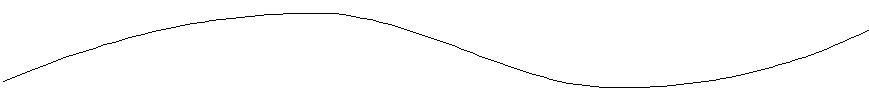
\includegraphics[width=\textwidth]{imgs/drawings/pwm/sinuois.png}
 \caption{The original sound.}
 \end{figure}
\par

\par
\begin{figure}[H]
\centering
 
\includegraphics[width=\textwidth]{imgs/drawings/pwm/pwm_approximation.png}
 \caption{The same sound approximated with square wave and frequency changes.}
 \end{figure}
\par

To do this, the audio system once again relies on the PIT chipset. Channel 0 is used to trigger the audio system. Channel 1 is used to refresh the RAM periodically. Channel 2, however, is directly connected to the PC Speaker. \\
\par
\begin{figure}[H]
  \centering
  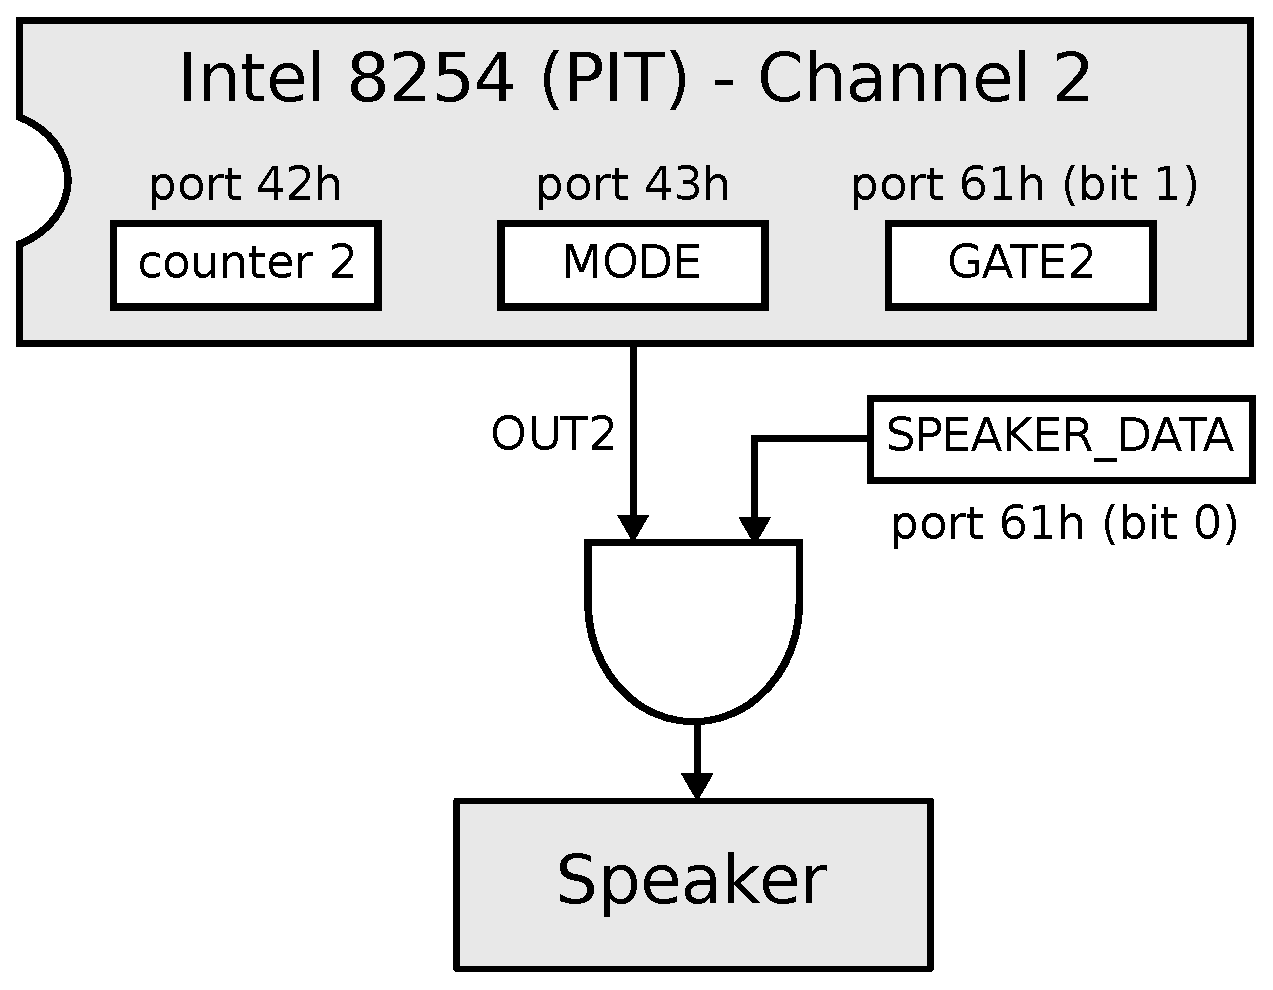
\includegraphics[width=0.65\textwidth]{imgs/drawings/pc_speaker.eps}
  \caption{Built-in speaker hardware diagram.}
  \label{fig:pc_speaker}
\end{figure}
\par

OUT2 is the output of Channel 2 of the PIT, GATE2 is the enable/trigger control for the Channel 2 counter, and SPEAKER\_DATA to control the speaker volume. The trick is to set OUT2 to square wave mode so it will repeat after it triggers and program the desired square wave frequency. This can be done by setting MODE in the PIT Command register to Mode 3.\\
\par
\begin{figure}[H]
\centering
   \begin{tabularx}{\textwidth}{ X X  }
	  \toprule
	  \textbf{Mode} & \textbf{Type} \\ \bottomrule
	    0 & Interrupt on Terminal Count\\
		1 & Hardware Re-triggerable One-shot\\
		2 & Rate Generator\\
		3 & Square Wave Generator\\
		4 & Software Triggered Strobe\\
		5 & Hardware Triggered Strobe\\
	  \bottomrule
  \end{tabularx}
  \caption{Available modes of a PIT counter.}
\end{figure}
\par 
When instructed to play a PC Speaker sound effect, the audio system sets itself to run at 140Hz via PIT Counter 0. Every times it wakes up, it reads the frequency to maintain for the next 1/140th of a second and writes it to Counter 2. The frequencies to use are encoded as a stream of bytes, the value of which is decoded as follows:\\
\par 
\begin{minipage}{\textwidth}
\lstinputlisting[language=C]{code/pwm.c}
\end{minipage}
\par

While the end result was not great, it was better than a beep.\\

\par
\begin{minipage}{\textwidth}
\lstinputlisting[language=C]{code/pwm_code.c}
\end{minipage}
\par

Notice how the \cw{* 60} is not calculated but looked up. Once again the engine tries to save as much CPU time as possible by using a bit of RAM. The frequency is read from a lookup table \cw{pcSoundLookup}.\\
\par
\begin{minipage}{\textwidth}
\lstinputlisting[language=C,morekeywords=word]{code/pcSoundLookup.c}
\end{minipage}
\par
Notice how \cw{0xb6} (\cw{10110110}) is sent to the PIC Command register:
\begin{itemize}
	\item \cw{10} = Target Counter 2.
 	\item \cw{11} = High \& low byte of counter updated.
	\item \cw{011} = (MODE) Square Wave Generator.
	\item \cw{0} = 16-bit mode.
\end{itemize}
\par




\end{document}










